\begin{figure}
\centering
    \begin{subfigure}{0.26\linewidth}
        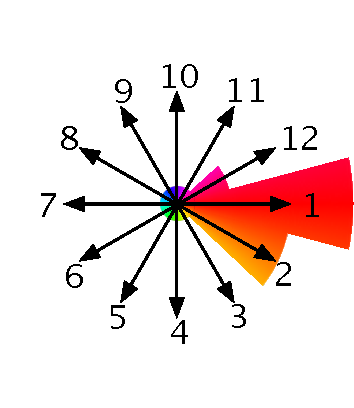
\includegraphics[width=\linewidth]{./img/scene_learning/grid_distribution.pdf}
        \subcaption{}
        \label{subfig:scene-grid-dist}
    \end{subfigure}
    \begin{subfigure}{0.35\linewidth}
        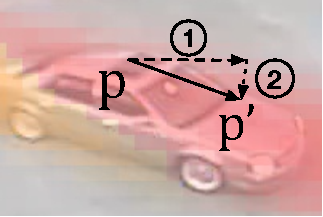
\includegraphics[width=\linewidth]{./img/scene_learning/step.pdf}
        \subcaption{}
        \label{subfig:scene-step}
    \end{subfigure}
    \begin{subfigure}{0.35\linewidth}
        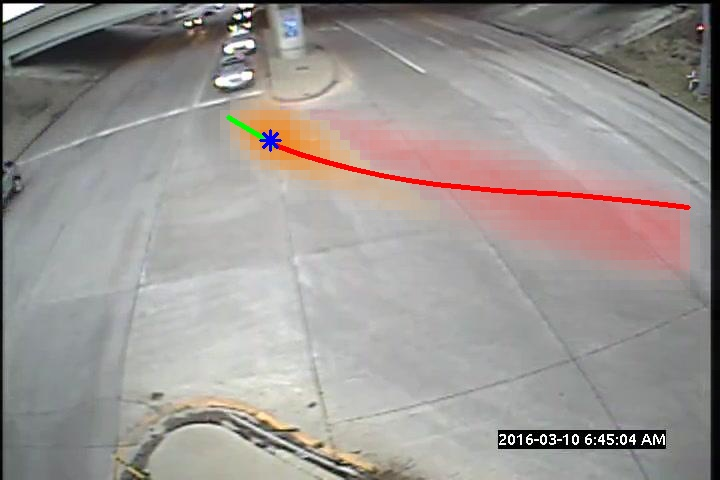
\includegraphics[width=\linewidth]{./img/scene_learning/single_ridge-1.jpg}
        \subcaption{}
        \label{subfig:scene-single-ridge}
    \end{subfigure}%
    \caption{\subref{subfig:scene-grid-dist} is an example of the topic distribution on one grid, where the radius of each circle sector indicates $\varphi_i^{1}$. \subref{subfig:scene-step} shows the move-adjust step of each iteration. \subref{subfig:scene-single-ridge} is an extracted ridge starting from the highest density grid, where the blue star indicates the highest density grid, green and red line indicates ridges to the start/end point separately.}
    \label{fig:scene-step}
\end{figure}